\appendix

\section{Detailed Data Tables}
\label{sec:appendix}

This appendix provides the full tabular data corresponding to figures
in the main text, as well as the original per-metric breakdowns that
were merged into Table~\ref{tab:apps_summary}.

\subsection{Application Benchmarks}

\begin{table}[h]
\caption{\textbf{\sys reduces RSS by 27--87\% with negligible throughput cost}
  (\S\ref{sec:eval:apps}).  Cool-phase RSS reduction.}
\label{tab:apps}
\centering\small
\begin{tabular}{lrrr}
\toprule
Application & RSS Reduction & Throughput & Cold p50 \\
\midrule
RocksDB         & \textbf{87.1\%}  & +2\%       & \textbf{0.8}\,$\mu$s \\
Redis           & 63.9\%  & \textbf{0\%}        & --- \\
Redis-ext       & 64.5\%  & \textbf{0\%}        & --- \\
SQLite          & 43.6\%  & $-$0.4\%   & 0.9\,$\mu$s \\
DuckDB          & 30.8\%  & \textbf{0\%}        & --- \\
Memcached       & 27.1\%  & \textbf{0\%}        & --- \\
\bottomrule
\end{tabular}
\end{table}

\begin{table}[h]
\caption{\textbf{Only \sys reduces RSS below fill level}
  (\S\ref{sec:eval:apps}).  Cool-phase RSS (MiB) across all six
  workloads.}
\label{tab:multi_alloc_apps}
\centering\small
\begin{tabular}{lrrrrrr}
\toprule
Allocator & SQLite & RocksDB & DuckDB & Redis & Redis-ext & Memcached \\
\midrule
System  & 424   & 434   & 1322  & 122  & 121  & 240 \\
Mesh    & 429   & 281   & 772   & 96   & 74   & 241 \\
\sys    & \textbf{239} & \textbf{56} & \textbf{915} & \textbf{44} & \textbf{43} & \textbf{175} \\
\bottomrule
\end{tabular}
\end{table}

\begin{figure}[h]
\centering
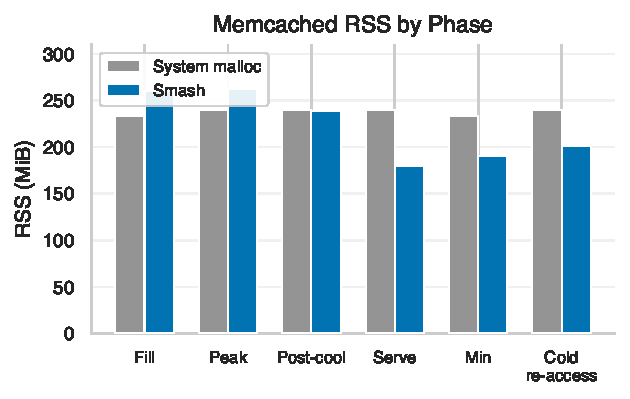
\includegraphics[width=\columnwidth]{figures/memcached.pdf}
\caption{\textbf{Memcached RSS drops 25\% during serve as idle
  data compresses} (\S\ref{sec:eval:apps}).  Fill-phase RSS is
  higher due to metadata overhead.}
\label{fig:memcached}
\end{figure}

\subsection{Algorithm Comparison}

\begin{table}[h]
\caption{\textbf{LZ4 and zstd compress real application heap pages well}
  (\S\ref{sec:eval:algo}).  Compression ratio =
  original\,/\,compressed (higher is better) on 16\,KiB heap pages
  sampled from each application.}
\label{tab:algo_compare}
\centering\small
\begin{tabular}{lrrrrr}
\toprule
Algorithm & SQLite & RocksDB & Memcached & Redis & DuckDB \\
\midrule
LZ4    & 12.3$\times$  & 8.6$\times$ & 4.7$\times$ & 6.3$\times$  & 2.1$\times$ \\
zstd-1 & 20.4$\times$  & 15.4$\times$ & 8.8$\times$ & 11.8$\times$ & 2.8$\times$ \\
zstd-3 & 20.4$\times$  & 15.6$\times$ & 9.3$\times$ & 11.9$\times$ & 2.9$\times$ \\
zstd-9 & \textbf{20.8$\times$} & \textbf{16.7$\times$} & \textbf{9.3$\times$} & \textbf{12.7$\times$} & \textbf{3.0$\times$} \\
\bottomrule
\end{tabular}
\end{table}

\subsection{Ablation Study}

\begin{table*}[h]
\caption{\textbf{Dictionaries hurt; compression is the dominant
  mechanism} (\S\ref{sec:eval:ablation}).  Default row: RSS
  reduction (\%); other rows: change in percentage points
  ($\Delta$\,\pp) from default.}
\label{tab:ablation}
\centering\small
\begin{tabular}{llrrrrr}
\toprule
 & Configuration & SQLite & RocksDB & Memcached & Redis & Avg.\ $\Delta$ \\
\midrule
    & \textbf{Default}  & \textbf{43.8\%}  & \textbf{87.1\%}  & \textbf{27.1\%} & \textbf{63.9\%} & --- \\
    & System malloc      & $-$17.6 & $-$80.3 & $-$42.3 & $-$42.3 & $-$45.6 \\
\midrule
    & With dicts         & $-$5.1  & $-$7.7  & $-$24.5 & $-$30.2 & $-$16.9 \\
    & No arenas          & 0.0     & $-$0.6  & $-$0.1  & $-$0.2  & $-$0.2 \\
    & LZ4 only           & 0.0     & $-$1.2  & 0.0     & $-$0.1  & $-$0.3 \\
    & No zero-deferred   & 0.0     & $-$1.5  & 0.0     & $-$0.2  & $-$0.4 \\
    & No prefetch        & 0.0     & $-$1.1  & 0.0     & +0.1    & $-$0.3 \\
    & Single worker      & 0.0     & $-$0.9  & +0.2    & +0.1    & $-$0.2 \\
    & No compression     & $-$20.3 & $-$80.3 & $-$40.0 & $-$42.3 & $-$45.7 \\
\bottomrule
\end{tabular}
\end{table*}

The dictionary adds only frame overhead ($\sim$13 bytes) without
improving ratios.  The effect is worst on memcached ($-$24.5\,\pp) and
Redis ($-$30.2\,\pp), where the CDict memory overhead exceeds the
small compressed-data savings.

RocksDB shows the largest marginal effects from individual
optimizations (1--2\,\pp) because its 16\,KiB block cache entries span
entire pages, making per-page optimizations more visible.

\subsection{Allocator Design Impact}

\begin{table}[h]
\caption{\textbf{Zero-on-free matters most on data with low
  byte-level redundancy (DuckDB); text-heavy workloads compress
  well regardless}
  (\S\ref{sec:eval:allocator}).  Compression ratio =
  original\,/\,compressed (higher is better) with zstd-9.
  $\dagger$Already zeroes on macOS.}
\label{tab:allocator_compare}
\centering\small
\begin{tabular}{lrrrr}
\toprule
Allocator & SQLite & Memcached & Redis & DuckDB \\
\midrule
\multicolumn{5}{l}{\textit{Base allocators}} \\
System malloc$^\dagger$ & 24.4$\times$ & \textbf{18.5$\times$} & 33.3$\times$ & \textbf{2.8$\times$} \\
mimalloc      & 24.4$\times$ & 13.5$\times$ & 33.3$\times$ & 1.5$\times$ \\
jemalloc      & 23.3$\times$ & 14.1$\times$ & \textbf{41.7$\times$} & 1.5$\times$ \\
tcmalloc      & 23.3$\times$ & 13.5$\times$ & 33.3$\times$ & 1.5$\times$ \\
Hoard         & \textbf{34.5$\times$} & 13.5$\times$ & 33.3$\times$ & 1.5$\times$ \\
Mesh$^\dagger$ & 24.4$\times$ & 18.2$\times$ & 33.3$\times$ & 2.8$\times$ \\
DieHard       & 40.0$\times$ & 11.6$\times$ & 31.3$\times$ & 1.6$\times$ \\
DieHarder     & \textbf{41.7$\times$} & \textbf{19.6$\times$} & \textbf{41.7$\times$} & \textbf{3.2$\times$} \\
\midrule
\multicolumn{5}{l}{\textit{With explicit zero-on-free}} \\
mimalloc+zero & 24.4$\times$ & 21.3$\times$ & 41.7$\times$ & 2.9$\times$ \\
jemalloc+zero & 23.3$\times$ & \textbf{23.8$\times$} & \textbf{55.6$\times$} & \textbf{3.0$\times$} \\
tcmalloc+zero & 23.3$\times$ & 20.8$\times$ & 43.5$\times$ & 2.9$\times$ \\
Hoard+zero    & \textbf{34.5$\times$} & 20.8$\times$ & 41.7$\times$ & 2.9$\times$ \\
DieHard+zero  & 40.0$\times$ & 19.6$\times$ & 41.7$\times$ & 3.2$\times$ \\
\sys          & \textbf{40.0$\times$} & 14.1$\times$ & 41.7$\times$ & 1.5$\times$ \\
\bottomrule
\end{tabular}
\end{table}

On DuckDB's columnar integer arrays---where freed slots contain stale
numeric data with no byte-level redundancy---allocators that do not
zero achieve only 1.5$\times$ compression (essentially incompressible
by LZ4), while allocators that zero achieve 2.8--3.2$\times$.  On
text-heavy workloads (memcached, Redis) the effect is smaller because
the data itself contains compressible patterns that dominate the
freed-slot noise.  DieHard+zero matches DieHarder exactly, confirming
that DieHarder's advantage comes entirely from its security zeroing.

We verified macOS zeroing by reading memory immediately after
\texttt{free}: 100\% of bytes are zeroed across all tested sizes
(32--4096\,B).  On workloads with frees, system malloc
(18.5$\times$ on memcached, 2.8$\times$ on DuckDB) outperforms
allocators that leave stale data in freed slots (mimalloc:
13.5$\times$, 1.5$\times$).

On SQLite (no frees), all allocators achieve 23--42$\times$
compression because every byte on the page is live, structured data.
The minor variation reflects differences in alignment padding and page
utilization, not metadata placement or zeroing~policy.

Note that \sys appears in the ``with zeroing'' section because
it defers zeroing to compression time (\S\ref{sec:design:zero});
in this static benchmark, the compressor is not running, so freed
slots retain stale data.  In production, the compressor zeros freed
slots in a scratch buffer immediately before compression, achieving
ratios comparable to the +zero~rows.
